\documentclass[hyperref={pdfencoding=unicode, unicode=true}]{beamer}
\usetheme{Berlin}

\usepackage[utf8x, utf8]{inputenc}
\usepackage{ucs}
\usepackage[english]{babel}
\usepackage{graphics}
\usepackage{booktabs}

\hypersetup{
	pdftitle={Acquisition of inflectional paradigms with minimal supervision},
	pdfauthor={Radoslav Klíč},
	pdfsubject={Acquisition of inflectional paradigms with minimal supervision}
}

\newcommand{\eg}{e.g.,~}

\title[Acquisition of inflectional paradigms]{Acquisition of inflectional paradigms with minimal supervision}
\author{Radoslav Klíč}
\institute{MFF UK}
\date{}

\begin{document}

%\AtBeginSection[]
%{
%  \begin{frame}<beamer>
%    \frametitle{Outline}
%    \tableofcontents[currentsection,currentsubsection]
%  \end{frame}
%}

\begin{frame}
\titlepage
\end{frame}

\begin{frame}{Outline}
	\tableofcontents
\end{frame}

\section{Introduction}

\begin{frame}{Introduction}

\begin{itemize}
\item The assignment: Acquisition of inflectional paradigms with minimal supervision
%plus slovnik
\item The approach: Modification and extension of an unsupervised paradigm learner
\end{itemize}

\end{frame}

\begin{frame}{}

Work done in the thesis:
\begin{itemize}
\item Modification of Paramor, an unsupervised morphology learner by Monson (2009),  to: \begin{itemize}
    \item accept manually provided inflections with marked morpheme boundary.
    \item handle allomorphy.
\end{itemize}
\item A framework for hierarchical clustering using modified edit distance and other string distance metrics.
\end{itemize}

\end{frame}

\section{Paramor}

\begin{frame}{Schemes}
\begin{itemize}
\item In Paramor, partial paradigms are modelled by \emph{schemes}. 
\item A scheme is defined by a set of its suffixes \eg (\emph{0, ed, ing, s}).
\item The scheme's stem set is obtained deterministically by selecting all the candidate stems which form a word (present in the corpus) with all the schemes suffixes.
\item Thus, adding a suffix can decrease the number of scheme's adherent stems (and cannot increase it). (More stems combine with (\emph{0, ed, ing, s}) than with (\emph{0, ed, ing, s, ly}))
\end{itemize}
\end{frame}

\begin{frame}{Scheme lattice}
\vspace{-8pt}
\begin{center}
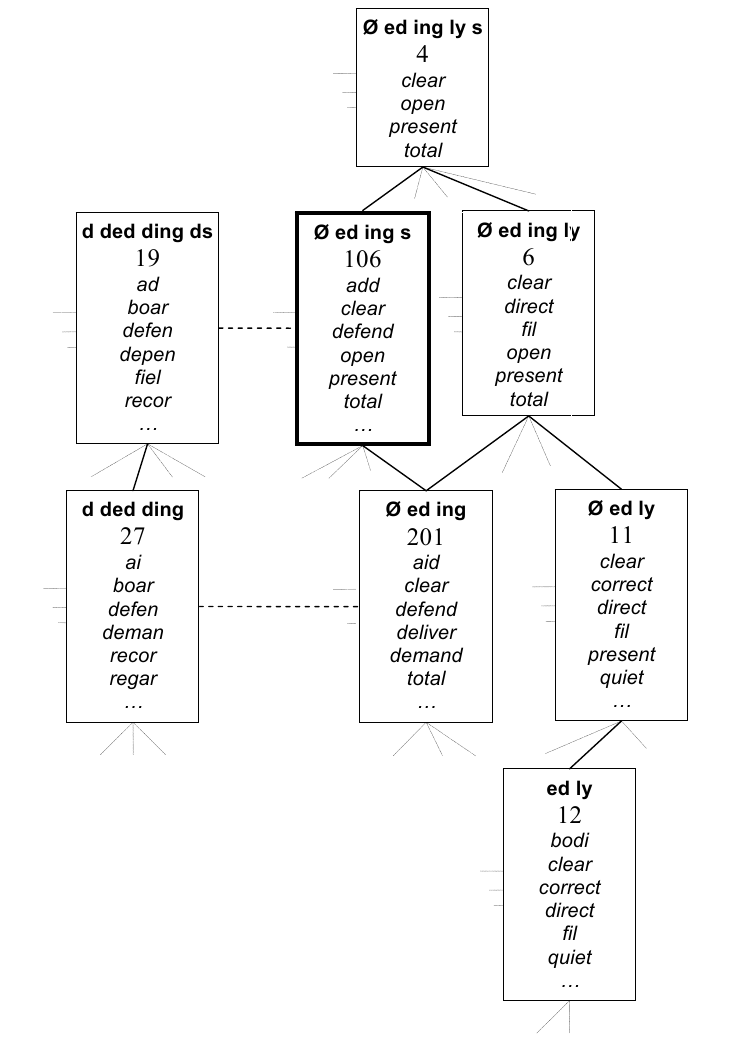
\includegraphics[scale=0.25]{schemeLattice.png}
\end{center}

\end{frame}


\begin{frame}{Paramor algorithm}
\begin{itemize}
\item Bottom-up search. Starts with single-suffix schemes and ascends the lattice. Stops when the c-stem ratio drops below 0.25.
\item Scheme clustering. Similar schemes are joined into scheme clusters. Similarity is defined as similarity of produced $<$stem, suffix$>$ pair sets. For example, schemes (\emph{0, ly, ness}) and (\emph{0, ly, er, est}) can be merged, as they share a lot of stem-suffix pairs like \emph{deep + 0}, \emph{deep + ly}.
\item Scheme cluster pruning.
\end{itemize}
\end{frame}

\section{Seeding}

\begin{frame}{Seeding}
\begin{itemize}
\item Seed example: \emph{matk/matc/matek} + \emph{a, u, y / e / 0}
\item Usage: \begin{itemize}
    \item Add two-suffix schemes to the initial scheme set for bottom-up search. The suffix pairs are taken from the manual seed. (I use pairs because schemes with larger subsets need not be present in the corpus)
    \item Protect some scheme clusters from discarding.
    \item Induction of allomorphy rules.
\end{itemize}
\end{itemize}
\end{frame}

\section{Allomorphy}

\begin{frame}{Allomorphy}
\begin{itemize}
\item Paramor does not recognise allomorphic stems. As a result, suffixes triggering phonological changes are often not selected in the bottom-up search, because they form words with different surface stems. 
\item I induce rules from the manual seed which allow Paramor to join two or more surface stems into one.
\item For example, from a seed entry 
\begin{quote}
\emph{politik/politic + a, u, ovi, em, y, ů, ům / i, ích}
\end{quote}
the following rule is generated:
\begin{quote}
$*k \leftrightarrow *c$ / \{\emph{a, u, ovi, em, y, ů, ům}\}, \{\emph{i, ích}\}
\end{quote}
\end{itemize}

\end{frame}

\section{Edit distance}

\begin{frame}{Edit distance}
In my clustering framework, I have experimented with modified Levenshtein distance, for which:
\begin{itemize}
\item the cost of operations linearly decreases with the position in the string where it occurs. (cost of \emph{walk} $\rightarrow$ \emph{talk} higher than \emph{talked} $\rightarrow$ \emph{talker})
\item the costs for diacritics adding/removing and vowel changes are lower than for other operations. (\emph{hranici} $\rightarrow$ \emph{hranicí}, \emph{žena} $\rightarrow$ \emph{ženy})
\end{itemize}
\end{frame}

\section{Results}

\begin{frame}{Evaluation}
\begin{itemize}
\item The subjects of evaluation are clusters of words which are compared to lexemes in a lemmatised corpus. (Lexeme -- set of all forms of one lemma.)
\item The evaluation method is pair-wise. For each pair of words, I check whether they belong to the same lemma and whether they belong to the same cluster created by the algorithm. I count true/false positives and true/false negatives and from them I get precision and recall to compute the F-score.
\end{itemize}
\end{frame}

\begin{frame}{Results}
\begin{center}
\begin{tabular}{lrrrr}
\toprule
\bf Corpus & \bf no seed & \bf seed & \bf edit & \bf noseed + edit \\
\midrule
cz & 69.63 & 72.74 & 61.89 & 72.26\\
si & 74.83 & 75.61 & 69.28 & 77.96\\
de & 60.12 & 60.13 & 64.87 & 63.28\\
cat & 62.74 & 65.95 & 56.50 & 63.91\\
\bottomrule
\end{tabular}
\end{center}
\end{frame}

\begin{frame}{Discussion}

Problems with German:

\begin{itemize}
\item Stem-internal changes (\emph{Mutter}/\emph{M\"{u}tter})

\item Compounds -- creation of schemes as (\emph{0, organisation}) or (\emph{0, gruppe})
\end{itemize}
\end{frame}

\begin{frame}{Future work}
\begin{itemize}

\item Rules for stem-internal vowel change (\emph{Mutter}/\emph{M\"{u}tter})

\item More information sources (context, semantics, \ldots)

\end{itemize}
\end{frame}


\end{document}